\documentclass{beamer}
\usepackage{listings}
\usetheme{Madrid}
\usecolortheme{seahorse}
\lstset{
%language=C,
frame=single, 
breaklines=true,
columns=fullflexible
}
\usepackage{subcaption}
\usepackage{url}
\usepackage{hyperref}
\usepackage{tikz}
\usepackage{amsmath}
\usepackage{graphicx}
\usepackage{tkz-euclide} % loads  TikZ and tkz-base
%\usetkzobj{all}
\usetikzlibrary{calc,math}
\usepackage{float}
\newcommand\norm[1]{\left\lVert#1\right\rVert}
\renewcommand{\vec}[1]{\mathbf{#1}}
\newcommand{\comb}[2]{{}^{#1}\mathrm{C}_{#2}}

\newcommand{\R}{\mathbb{R}}
\newcommand{\C}{\mathbb{C}}
\newcommand{\Beta}{B}
\newcommand{\Int}{\int\limits}
\providecommand{\brak}[1]{\ensuremath{\left(#1\right)}}
\providecommand{\abs}[1]{\vert#1\vert}
\providecommand{\fourier}{\overset{\mathcal{F}}{ \rightleftharpoons}}
\providecommand{\pr}[1]{\ensuremath{\Pr\left(#1\right)}}
\providecommand{\sbrak}[1]{\ensuremath{{}\left[#1\right]}}
\usepackage[export]{adjustbox}
\usepackage[utf8]{inputenc}
\usepackage{amsmath}
%environment for large proof
\makeatletter
\newenvironment<>{proofs}[1][\proofname]{%
    \par
    \def\insertproofname{#1\@addpunct{.}}%
    \usebeamertemplate{proof begin}#2}
  {\usebeamertemplate{proof end}}
\makeatother

\title{Order Statistics}
\subtitle{GATE 2021 (ST), Q.17 (STATISTICS SECTION)}
\author{Suraj Telugu - CS20BTECH11050}
\institute{IITH}
\date{\today}
\begin{document}
%
\begin{frame}
\titlepage
\end{frame}
%slide 2
\begin{frame}{Topics covered:}
\begin{block}{Prerequisites:}
\begin{enumerate}[]
\item Definition of order statistics 
\item Range, median and an example
\item Theorem 1 and its proof  (CDF of $k^{th}$ order statistic)
\item Theorem 2 and its proof  (PDF of $k^{th}$ order statistic)
\item Uniform order statistics 
\item Introducing Beta function
\item Beta distribution and its features
\end{enumerate}
\end{block}
\begin{block}{Gate Problem}
\begin{enumerate}[]
 \item Problem
\item Solution method 1
\item Solution method 2
\end{enumerate}
\end{block}
\end{frame}
%slide 3
\begin{frame}{Introduction to Order statistics}
\begin{block}{Definition}
\begin{enumerate}[]
\item
For a given statistical sample $\{X_1, X_2,\cdots X_n\}$, The order statistics is obtained by sorting the sample in ascending order
\item The ordered sample values are denoted as $\{X_{(1)}, X_{(2)},\cdots X_{(n)}\}$
\item $X_{(1)}$ is the minimum and $X_{(n)}$ is the maximum of the given sample
\item The $k^{th}$ smallest value $X_{(k)}$ is called  $k^{th}$ order statistic 
\begin{align}
X_{(1)} &\leq X_{(2)}\leq \cdots\leq X_{(k)}\leq \cdots \leq X_{(n)} 
\end{align}
\item For a sample $\{X_1, X_2, \cdots X_n\}$ of size n:
    \begin{align}
        X_{(k)} = \min\{\max\{X_{j}:j\in J\}\,:\,J\subset\{1,2\cdots n\}\;|J| = k\}
    \end{align}
\end{enumerate}
 \end{block}
\end{frame}
%slide 4
\begin{frame}{Introduction to Order statistics}
\begin{block}{Range and Median}
\begin{enumerate}[]
\item For a sample $\{X_1, X_2, \cdots X_n\}$, the range is the distance between the smallest and largest observations and is denoted by $R$
\begin{align}
   R = X_{(n)}-X_{(1)}
\end{align}
        
\item Median is as the middle number of a sorted sample it is denoted by M it is defined using order statistics of a sample as
\begin{align}
  M =
  \begin{cases}
   X_{((n+1)/2)},                                           &\text{if $n$ is odd,} \\ \\
  \dfrac{ X_{(n/2)} + X_{(n/2+1)}}{2} ,                     &\text{if $n$ is even,} 
  \end{cases}
\end{align}
\end{enumerate}
\end{block}
\end{frame}
%slide 5
\begin{frame}{Introduction to Order statistics}
\begin{block}{Example Problem}
For the given data sample $\{1,7,11,5,-4\}$ discuss the order statistics and 
find the  value of $2^{nd}$ order statistic, range and median 
 \begin{align}
X_{(1)} = -4, 
X_{(2)} = 1,
X_{(3)} = 5,
X_{(4)} = 7,
 X_{(5)} = 11
 \end{align}
 \begin{align}
2^{nd} \text{Order statistic} &= 1 \\
\text{Range} =  R = X_{(5)} - X_{(1)} &= 15 \\
\text{Median} = M = X_{(3)}  &= 5
 \end{align}
 \begin{figure}
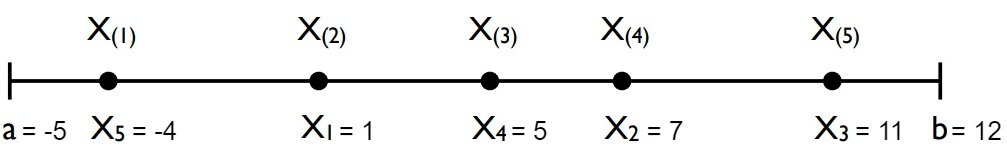
\includegraphics[max size={0.9\textwidth}{0.2\textheight}]{num_line.png}
\end{figure}
\end{block}
\end{frame}
%slide 6
\begin{frame}{CDF of $k^{th}$ order statistic}

\begin{theorem}[1]
Let $\{X_1, X_2, \cdots X_n\}$ be n i.i.d random variables with common CDF $= F(x)$ and common PDF $= f(x)$, 
then the marginal probability distribution of $k^{th}$ order statistic (CDF) is denoted by $F_{(k,n)}(x)$ 
and it is given by
\begin{align}
CDF = F_{(k,n)}(x) =  \sum_{j=k}^{n}\comb{n}{j}\times \brak{F(x)}^{j}\times\brak{1-F(x)}^{n-j} \label{eqn_1}
\end{align}
\label{th1}
\end{theorem}
\begin{block}{Extreme cases}
    Equation \eqref{eqn_1} gives $X_{(1)}$ and $X_{(n)}$ as:
\begin{align}
\text{Distribution of minimum} &= F_{(1,n)}(x) =1-(1-F(x))^n\\
\text{Distribution of maximum} &= F_{(n,n)}(x) =(F(x))^n
\end{align}
\end{block}
\end{frame}
%slide 7
\begin{frame}{Proof of theorem \eqref{th1}:}
\begin{proofs}[Theorem \eqref{th1} Proof]
Assume after order statistics, the sample becomes $\{X_{(1)}, X_{(2)}\cdots X_{(n)}\}$ 
we need to find $F_{(k,n)}(x)=\pr{X_{(k)}\leq x}$
\begin{align}
X_{(i)} &\leq X_{(k)} \leq x\;\forall i \in \{1,\cdots k-1\} \label{eqn_4} \\
X_{(i)} &\leq x \text{  or  } X_{(i)} > x \;\forall i \in \{k+1,\cdots n\} 
\end{align}
From the above equation \eqref{eqn_4}, at least $k$ elements in $\{X_{1}, X_{2}\cdots X_{n}\}$ 
should be $\leq x$ and remaining $(n-k)$ elements can be $\leq x$ or $> x$
\begin{align}
F_{(k,n)}(x) &= \pr{\text{At least k elements have value $\leq x$}} \\
F_{(k,n)}(x) &= \pr{X_i \leq x\,:\,i\in I\,:\,I\subset\{1,\cdots n\}\;|I|\geq k}
\end{align}
\end{proofs}
\end{frame}
%slide 8
\begin{frame}{Proof of theorem \eqref{th1}:}
\begin{proof}[Theorem \eqref{th1} Proof contd]
\begin{multline}
F_{(k,n)}(x) =\comb{n}{k}\pr{X\leq x}^{k}\pr{X>x}^{n-k} + \\
\comb{n}{k+1}\pr{X\leq x}^{k+1}\pr{X>x}^{n-(k+1)} +  \\
\cdots \cdots \comb{n}{n}\pr{X\leq x}^{n}\pr{X>x}^{0}
\end{multline}
\begin{align}
F_{(k,n)}(x) &=\sum_{j=k}^{n}\comb{n}{j} \pr{X\leq x}^{j}\pr{X>x}^{(n-j)} \\
\therefore F_{(k,n)}(x) &=  \sum_{j=k}^{n}\comb{n}{j}\times \brak{F(x)}^{j}\times\brak{1-F(x)}^{n-j} 
\end{align}
\end{proof}
\end{frame}
%slide 9
\begin{frame}{PDF of $k^{th}$ order statistic}
\begin{theorem}[2]
Let $\{X_1, X_2, \cdots X_n\}$ be n i.i.d random variables with common CDF $= F(x)$ and common PDF $= f(x)$, 
then the marginal probability density of $k^{th}$ order statistic (PDF) is denoted by $f_{(k,n)}(x)$  and it
is given by
\begin{align}
PDF = f_{(k,n)}(x) = n\;\comb{n-1}{k-1}\,f(x)\,(F(x))^{k-1}\,\brak{1-F(x)}^{n-k} \label{eqn_2}
\end{align}
\label{th2}
\end{theorem}
\begin{block}{Extreme cases}
Equation \eqref{eqn_2} gives $X_{(1)}$ and $X_{(n)}$ as:
\begin{align}
\text{Density of minimum} &= f_{(1,n)}(x) = n\,f(x)\,(1-F(x))^{n-1} \\
\text{Density of maximum} &= f_{(n,n)}(x) = n\,f(x)\,(F(x))^{n-1}
\end{align}
\end{block}
\end{frame}
%slide 10
\begin{frame}{Proof of theorem \eqref{th2} in a simpler way:}
\begin{proof}[Theorem \eqref{th2} Proof]
let us assume $X_{(k)}\in[x,x+dx]$ for $dx \to 0$. Solving using 4 sub -jobs
\begin{align}
\text{Job 1} &= \text{Choose $X_i=X_{(k)}$ and \pr{X_i\in[x,x+dx]}} = \comb{n}{1}f(x) \\
\text{Job 2} &= \text{Choose $k-1$ elements from remaining} = \comb{n-1}{k-1} \\
\text{Job 3} &= \pr{X\leq x} \text{for chosen $(k-1)$ elements} = {F(x)}^{k-1} \\
\text{Job 4} &=  \pr{X > x} \text{for $(n-k)$ elements}  = (1-F(x))^{n-k} 
\end{align}
\begin{equation}
\pr{X_{(k)}\in[x,x+dx]} = f_{(k,n)}(x) = \prod_{i=1}^{4} \text{Job i} 
\end{equation}
\begin{align}
 \therefore f_{(k,n)}(x) =  n\;\comb{n-1}{k-1}\,f(x)\,(F(x))^{k-1}\,\brak{1-F(x)}^{n-k}
\end{align}
\end{proof}
\end{frame}
%slide 11
\begin{frame}{Uniform order statistics}
\begin{block}{Introduction}
Let $\{X_1,\cdots X_n\}$ be i.i.d form a uniform distribution on $[0,1]$ such that $f(x) = 1$ and $F(x)=x$,
from theorem \eqref{th2}, equation \eqref{eqn_2}
\begin{align}
f_{(k,n)}(x) &= n\;\comb{n-1}{k-1}\,f(x)\,(F(x))^{k-1}\,\brak{1-F(x)}^{n-k} \label{eqn_6} \\
f_{(k,n)}(x) &= n\;\comb{n-1}{k-1}\,x^{k-1}\,\brak{1-x}^{n-k} \label{eqn_3}
\end{align}
Since equation \eqref{eqn_3} is marginal probability density (PDF) 
\begin{align}
\Int_{0}^{1} n\;\comb{n-1}{k-1}\,x^{k-1}\,\brak{1-x}^{n-k} \,dx  &= 1   \\
\Int_{0}^{1} x^{k-1}\,\brak{1-x}^{n-k} \,dx  &= \dfrac{1}{n\;\comb{n-1}{k-1}} 
\end{align}
\end{block}
\end{frame}
%slide 12
\begin{frame}{Uniform order statistics}
\begin{block}{Introduction contd}
\begin{align}
\Int_{0}^{1} x^{k-1}\,\brak{1-x}^{n-k} \,dx  &= \dfrac{(k-1)!\,(n-k)!}{n!}  \\
\Int_{0}^{1} x^{k-1}\,\brak{1-x}^{n-k} \,dx  &= \dfrac{\Gamma(k)\,\Gamma(n-k+1)}{\Gamma\brak{(n-k+1)+k)}} 
\end{align}
\end{block}
\begin{definition}
let $r = k$ and $s = n-k+1$ The \textbf{Beta function} is defined for r, s $> 0$
\begin{equation}
\Beta(r,s) = \Int_{0}^{1} x^{r-1}\,\brak{1-x}^{s-1}\,dx = \dfrac{\Gamma(r)\,\Gamma(s)}{\Gamma(r+s)} \label{eqn_5}
\end{equation}
\end{definition}
\end{frame}
%slide 13
\begin{frame}{Beta function}
\begin{block}{Substituting in equation \eqref{eqn_6} and \eqref{eqn_3}}
By using the above definition and equation 
\begin{align}
f_{(k,n)}(x) &= \dfrac{1}{\Beta(k,n-k+1)}\,f(x)\,(F(x))^{k-1}\,\brak{1-F(x)}^{n-k} \\
f_{(k,n)}(x) &= \dfrac{x^{k-1}\,\brak{1-x}^{n-k}}{\Beta(k,n-k+1)}\;\text{(Uniform order statistics)} \label{eqn_7}
\end{align}
\end{block}
\begin{block}{Beta distribution}
The Beta distribution is a continuous distribution defined on the range $(0,1)$ whose PDF given by 
\begin{align}
f(x) &= \dfrac{1}{\Beta(r,s)}\,x^{r-1}\,\brak{1-x}^{s-1} 
\end{align}
\end{block}
\end{frame}
%slide 14
\begin{frame}{Beta Distribution}
\begin{block}{Beta distribution contd}
Let $\Beta_{x}(r,s)=\Int_{0}^{x} x^{r-1}\,\brak{1-x}^{s-1}\,dx$, CDF of Beta distribution:
\begin{align}
 F(x) &= \Int_{0}^{x}f(x)\,dx  = \Int_{0}^{x}\dfrac{1}{\Beta(r,s)}\,x^{r-1}\,\brak{1-x}^{s-1}\,dx  \\
 F(x) &=  \dfrac{\Int_{0}^{x} x^{r-1}\,\brak{1-x}^{s-1}\,dx}{\Beta(r,s)} = \dfrac{\Beta_{x}(r,s)}{\Beta(r,s)}\\
\end{align}
\begin{equation}
 \therefore \text{CDF} = F(x) = \dfrac{\Beta_{x}(r,s)}{\Beta(r,s)}
\end{equation}
\end{block}
\end{frame}
%slide 15
\begin{frame}{Beta distribution}
\begin{block}{Mean value of Beta distribution}
\begin{align}
 E(x)  &= \Int_{0}^{1}x\times f(x)\,dx = \Int_{0}^{1}\dfrac{x}{\Beta(r,s)}\,x^{r-1}\,\brak{1-x}^{s-1}\,dx \\
       &= \dfrac{\Int_{0}^{1} x^{(r+1)-1}\,\brak{1-x}^{s-1}\,dx}{\Beta(r,s)} = \dfrac{\Beta(r+1,s)}{\Beta(r,s)} \\
       &= \dfrac{\Gamma(r+1)\,\Gamma(s)}{\Gamma(r+s+1)} \times \dfrac{\Gamma(r+s)}{\Gamma(r)\,\Gamma(s)} \\
       &= \dfrac{r!}{(r+s)!} \times \dfrac{(r+s-1)!}{(r-1)!} = \dfrac{r}{r+s}
\end{align}
\begin{equation}
\therefore \text{Mean value of X $(E(x))$} = \dfrac{r}{r+s}
\end{equation}
\end{block}
\end{frame}
%slide 16
\begin{frame}{Beta distribution}
\begin{block}{Variance of Beta distribution}
\begin{align}
 Var(x) &= E(x^{2}) - (E(x))^2 \\
&=  \dfrac{\Int_{0}^{1} x^{(r+2)-1}\,\brak{1-x}^{s-1}\,dx}{\Beta(r,s)} - \brak{\dfrac{r}{r+s}}^{2} \\
&=  \dfrac{\Beta(r+2,s)}{\Beta(r,s)} - \dfrac{r^2}{(r+s)^2} \\
&= \dfrac{\Gamma(r+2)\,\Gamma(s)}{\Gamma(r+s+2)} \times \dfrac{\Gamma(r+s)}{\Gamma(r)\,\Gamma(s)} -\dfrac{r^2}{(r+s)^2}   \\
&=  \dfrac{(r+1)!}{(r+s+1)!} \times \dfrac{(r+s-1)!}{(r-1)!} - \dfrac{r^2}{(r+s)^2}  
\end{align}
\end{block}
\end{frame}
%slide 17
\begin{frame}{Beta Distribution}
\begin{block}{Variance of Beta distribution contd}
\begin{align}
 &=  \dfrac{r(r+1)}{(r+s)(r+s+1)} - \dfrac{r^2}{(r+s)^2} \\
 &=  \dfrac{r(r+1)(r+s) - r^2(r+s+1)}{(r+s)^2(r+s+1)} \\
 &=  \dfrac{(r^3+r^{2}s+r^{2}+rs) - (r^3+r^{2}s+r^{2}))}{(r+s)^2(r+s+1)} \\
 Var(x) &= \dfrac{rs}{(r+s)^{2}(r+s+1)}
\end{align}
\begin{equation}
\therefore \text{Variance of X ($Var(x)$)} =  \dfrac{rs}{(r+s)^{2}(r+s+1)}
\end{equation}
\end{block}
\end{frame}
%slide 18
\begin{frame}{Beta Distribution}
\begin{block}{Beta distribution summary}
PDF, CDF, Expectation value and Variance of Beta distribution
\begin{align}
 f(x)   &= \dfrac{1}{\Beta(r,s)}\,x^{r-1}\,\brak{1-x}^{s-1} \\
 F(x)   &=   \dfrac{\Beta_{x}(r,s)}{\Beta(r,s)} \\
 E(x)   &=   \dfrac{r}{r+s} \\
 Var(x) &= \dfrac{rs}{(r+s)^{2}\,(r+s+1)}
\end{align}
In Uniform order statistics on [0,1] the PDF of $k^{th}$ order statistic follows Beta distribution with $r=k$, $s=n-k+1$ and PDF
$f_{(k,n)}(x)$  from the above equation \eqref{eqn_7}
\end{block}
\end{frame}
%slide 19
\begin{frame}{Gate problem}
\begin{block}{GATE 2021 (ST), Q.17 (STATISTICS SECTION)}
If the marginal probability density function of the $k^{th}$ order statistic of a 
random sample of size 8 from a uniform distribution on $[0,2]$ is
\[
  f(x) =
  \begin{cases}
   \dfrac{7}{32}\,x^{6}\,\brak{2-x},  & 0<x<2, \\ 
      \hspace{1cm}   0,               & \text{otherwise,} 
  \end{cases}
\]
then $k$ equals \underline{\hspace{3cm}}
\end{block}
\end{frame}
%slide 20
\begin{frame}{Solution (Using Theorem\eqref{th2})}
\textbf{Method 1:}\\
The problem involves the uniform order statistics on $[0,2]$, sample size 8, we begin the solution by finding the PDF of the given sample:
\begin{align}
\Int_{0}^{2}f(x)\,dx &= 1   \\
            f(x) &= \dfrac{1}{2} \label{pdf}
\end{align}
CDF of the given sample:
\begin{equation}
F(x) = \Int_{0}^{x}f(x)\,dx = \dfrac{x}{2} \label{cdf}
\end{equation}
\end{frame}
%slide 21
\begin{frame}{Solution (Using Theorem\eqref{th2})}
Using Theorem \eqref{th2} PDF of $k^{th}$ order statistic is given by 
\begin{align}
f_{(k,n)}(x) &= n\;\comb{n-1}{k-1}\,f(x)\,(F(x))^{k-1}\,\brak{1-F(x)}^{n-k} \\
f_{(k,n)}(x) &= n\;\comb{n-1}{k-1}\,\dfrac{1}{2}\,\brak{\dfrac{x}{2}}^{k-1}\,\brak{1-\dfrac{x}{2}}^{n-k} \\
f_{(k,8)}(x) &= \dfrac{8}{2^{(1+(k-1)+(8-k))}}\times\comb{7}{k-1}\,x^{k-1}\,\brak{2-x}^{8-k}\\
f_{(k,8)}(x) &= \comb{7}{k-1}\,\dfrac{1}{32}\,x^{k-1}\,\brak{2-x}^{8-k} \label{eqn_8}
\end{align}
Comparing equation \eqref{eqn_8} with the given PDF of $k^{th}$ order statistic
\begin{align}
\dfrac{\comb{7}{k-1}}{32}\,x^{k-1}\,\brak{2-x}^{n-k} &= \dfrac{7}{32}\,x^{6}\,\brak{2-x} \\
\therefore k = 7 
\end{align}
\end{frame}
%slide 22
\begin{frame}{PDF and CDF of Uniform Distribution}
The plots of PDF, CDF of uniform statistics in equations \eqref{pdf} and \eqref{cdf}:
 \begin{figure}%
    \centering
    \subfloat[\centering PDF $f(x)$]{{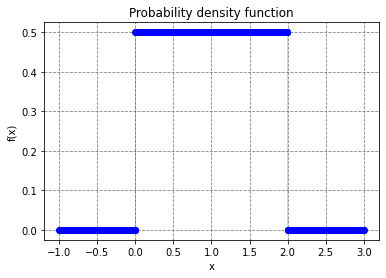
\includegraphics[width=5.5cm]{PDF.png} }}%
    \qquad
    \subfloat[\centering CDF $F(x)$]{{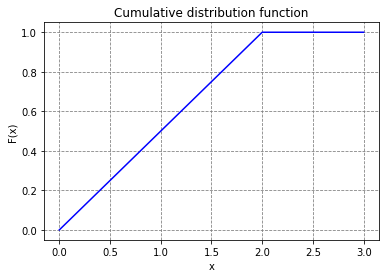
\includegraphics[width=5.5cm]{CDF.png} }}%
    \caption{PDF and CDF of given uniform statistics}%
    \label{fig:example 2}%
 
\end{figure}
\end{frame}
%slide 23
\begin{frame}{Solution(Using Beta distribution)}
\textbf{Method 2:}\\
Since the $k^{th}$ order statistic of a uniform distribution on $[0,1]$ follows Beta distribution, convert 
the random variables, given PDF in $[0,1]$ range 
\begin{align}
\Int_{0}^{2}f(x)\,dx &= \Int_{0}^{2} \dfrac{7}{32}\,x^{6}\,\brak{2-x}\,dx \\
\Int_{0}^{2}f(x)\,dx &= \Int_{0}^{2} 56\,\brak{\dfrac{x}{2}}^{6}\,\brak{1-\dfrac{x}{2}}\,d\brak{\dfrac{x}{2}} 
\end{align}
\begin{equation}
\text{Let, } f_{(k,8)}(t) = 56\,t^{6}\,\brak{1-t}
\end{equation}
Let new random variable be $t$ such that $t=x/2$, New sample be $\{T_1,\cdots T_8\}$ such that $T_{i}=X_{i}/2$.
\end{frame}
%slide 24
\begin{frame}{Solution(Using Beta distribution)}
The Uniform distribution of new random sample is on $[0,1]$ such that $f(t)=1$ and $    F(t)=t$ 
\begin{align}
\Int_{0}^{2}f(x)\,dx &= \Int_{0}^{1} 56\,t^{6}\,(1-t)\,dt = \Int_{0}^{1}f(t)\,dt
\end{align}
Given $k^{th}$ order statistic (after conversion)
\begin{align}
f_{(k,8)}(t) =
  \begin{cases}
      56\,t^{6}\,\brak{1-t},  & 0<t<1, \\ 
      \hspace{1cm}   0,               & \text{otherwise,} 
  \end{cases}
  \label{eqn_9}
\end{align}
Since equation \eqref{eqn_9} is a Beta distribution with $r=k$, $s=n-k+1$ 
\begin{align}
k-1 &= 6 \\
\therefore k = 7 
\end{align}
\end{frame}
%slide 25
\begin{frame}{Plots of PDF of $k^{th}$ order statistic}
The plots for given PDF and PDF in equation \eqref{eqn_9} are shown below:
 \begin{figure}%
    \centering
    \subfloat[\centering PDF of $f_{(7,8)}(x)$]{{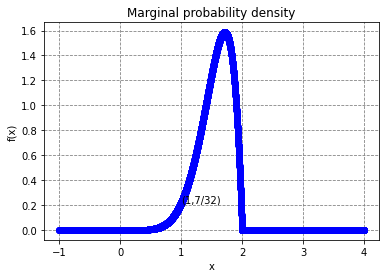
\includegraphics[width=5.5cm]{MPD_1.png} }}%
    \qquad
    \subfloat[\centering PDF of $f_{(7,8)}(t)$]{{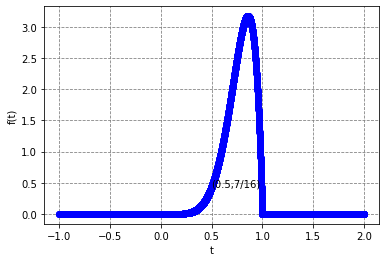
\includegraphics[width=5.5cm]{MPD_2.png} }}%
    \caption{Plots of $k^{th}$ order statistic}%
    \label{fig:example 1}%
 
\end{figure}
\end{frame}


\begin{frame}
   \centering
    \textcolor{blue}{\Huge{\textbf{THANK YOU}}} 
\null \par \null
\textcolor{orange}{\textbf{Assignment link for reference: }}\\
\url{https://github.com/Suraj11050/Assignments-AI1103/tree/main/Assignment 4}
\end{frame}

\end{document}

